%! alt Right-angled triangle ABC with the right angle at C, AC = 30, BC = 40 and hypotenuse AB = 50, drawn with AB horizontal. D is the foot of the perpendicular from C to AB, with AD = 18 and CD = 24. The incircles of triangles ACD and BCD are drawn, with radii 6 and 8.
%! after_paragraph 2
%! scale 1/9
% The shared preamble of every Cevian figure. pipeline/figures turns these colours into theme-aware paint,
% and refuses any other colour, so draw only with them:
%   figink (lines and labels), figaux (construction lines), figaccent (the object the argument turns on),
%   figtint and figaccenttint (light fills).
\documentclass[border=1.5pt]{standalone}
\usepackage{tkz-euclide}
\definecolor{figink}{RGB}{0,0,0}
\definecolor{figaux}{RGB}{85,85,85}
\definecolor{figaccent}{RGB}{192,57,43}
\definecolor{figtint}{RGB}{221,221,221}
\definecolor{figaccenttint}{RGB}{245,213,208}
% tkz-euclide's defaults draw circles, compasses and marks in 50% grey and fill points with a tint.
\makeatletter
\def\tkz@otherlinecolor{figink}
\def\tkz@euc@circlecolor{figink}
\def\tkz@euc@compasscolor{figink}
\def\tkz@euc@mkcolor{figink}
\def\tkz@mk@fill{figink}
\def\tkz@euc@pointfillcolor{figink}
\makeatother
\tkzSetUpLine[color=figink,line width=.7pt]
\tkzSetUpArc[color=figink,line width=.7pt]
\tkzSetUpCompass[color=figink,line width=.5pt]
\tkzSetUpPoint[color=figink,fill=figink,size=3.1pt]
\tikzset{
  every picture/.style={line cap=round,line join=round,color=figink},
  circle style/.append style={color=figink,line width=.7pt},
  aux/.style={color=figaux,line width=.45pt,dash pattern=on 2.6pt off 2pt},
  key/.style={color=figaccent,line width=1pt},
  mk/.style={color=figink,line width=.5pt},
  lbl/.style={color=figink,inner sep=2.2pt},
  len/.style={color=figink,inner sep=1.5pt,font=\small},
}

\begin{document}
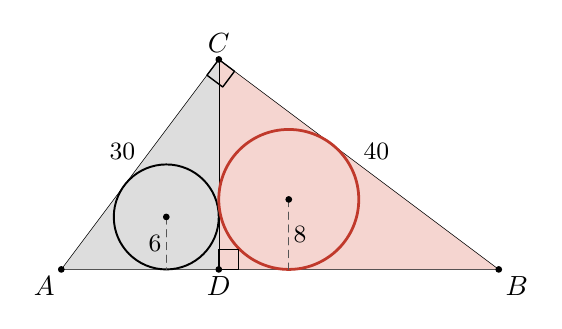
\begin{tikzpicture}
\tkzDefPoint(0.0,0.0){A} %! A = (0, 0)
\tkzDefPoint(5.5555556,0.0){B} %! B = (50, 0)
\tkzDefPoint(2.0000000,2.6666667){C} %! C = (18, 24)
\tkzDefPoint(2.0000000,0.0){D} %! D = (18, 0)
\tkzDefPoint(1.3333333,0.66666667){I} %! I = incentre(A, C, D)
\tkzDefPoint(2.8888889,0.88888889){J} %! J = incentre(B, C, D)
\tkzDefPoint(1.3333333,0.0){S} %! S = foot(I, A, D)
\tkzDefPoint(2.8888889,0.0){T} %! T = foot(J, B, D)
%! fact perp(A, C, C, B)
%! fact perp(C, D, A, B)
%! fact inradius(A, C, D) == 6
%! fact inradius(B, C, D) == 8
%! fact dist(I, S) == 6
%! fact dist(J, T) == 8
%! fact dist(A, C) == 30
%! fact dist(B, C) == 40
%! fact dist(A, B) == 50
\tkzFillPolygon[color=figtint](A,C,D)
\tkzFillPolygon[color=figaccenttint](B,C,D)
\tkzDrawPolygon(A,B,C)
\tkzDrawSegment(C,D)
\tkzDrawCircle(I,S)
\tkzDrawCircle[key](J,T)
\tkzDrawSegments[aux](I,S J,T)
\tkzMarkRightAngle[size=.25,mk](A,C,B)
\tkzMarkRightAngle[size=.25,mk](C,D,B)
\tkzDrawPoints(A,B,C,D,I,J)
\tkzLabelPoint[below left,lbl](A){$A$}
\tkzLabelPoint[below right,lbl](B){$B$}
\tkzLabelPoint[above,lbl](C){$C$}
\tkzLabelPoint[below,lbl](D){$D$}
\tkzLabelSegment[left,len](I,S){$6$}
\tkzLabelSegment[right,len](J,T){$8$}
\tkzLabelSegment[above left,len](A,C){$30$}
\tkzLabelSegment[above right,len](B,C){$40$}
\end{tikzpicture}
\end{document}
